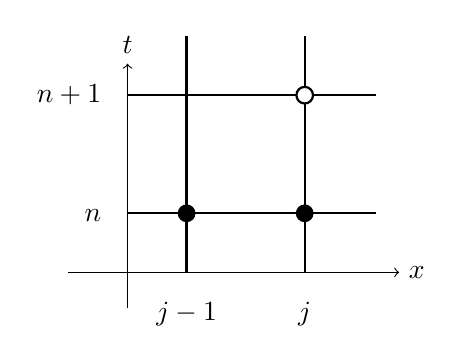
\begin{tikzpicture}[
    fdot/.style={circle, fill=black, draw=black, minimum size=6pt, inner sep=0pt},
    odot/.style={circle, fill=white, draw=black, line width=0.8pt, minimum size=6pt, inner sep=0pt}
]
\pgfmathsetmacro{\dx}{1.5}
\pgfmathsetmacro{\dt}{1.5}
\pgfmathsetmacro{\sep}{5.8}

%% upwind (right, c>0)
\draw[thick] (-1.5*\dx,0) -- (0.6*\dx,0);
\draw[thick] (-1.5*\dx,\dt) -- (0.6*\dx,\dt);
\draw[thick] (-\dx,-0.75) -- (-\dx,1.5*\dt);
\draw[thick] (0,-0.75)    -- (0,1.5*\dt);
%\draw[thick] (\dx,-0.75)  -- (\dx,1.5*\dt);
\node[fdot] at (-\dx,0) {};
\node[fdot] at (0,0)    {};
%\node[fdot] at (\dx,0)  {};
\node[odot] at (0,\dt)  {};
\node[below] at (-\dx,-1) {$j-1$};
\node[below] at (0,-1)    {$j$};
%\node[below] at (\dx,-1)  {$j+1$};
\node[left=6pt]  at (-1.5*\dx,0)   {$n\vphantom{+1}$};
\node[left=6pt]  at (-1.5*\dx,\dt) {$n+1$};
\draw[->] (-2*\dx,-0.75) -- (0.8*\dx,-0.75) node[right] {$x$};
\draw[->] (-\dx-0.75,-1.2) -- (-\dx-0.75,\dt+0.4) node[above] {$t$};
\end{tikzpicture}
